\documentclass{beamer}

\setbeamertemplate{navigation symbols}{}
\setbeamertemplate{footline}[frame number]

% no numbers
\setbeamerfont{footnote}{size=\tiny}
\setbeamertemplate{footnote}{%
  \parindent 1em\noindent%
  \raggedright
  \insertfootnotetext\par%
}

\usepackage{graphicx}
\usepackage{chemfig}
\usepackage{tikz}
\usetikzlibrary{calc}
\usepackage{hyperref}
\hypersetup{
  colorlinks=true,
  linkcolor=blue,
  filecolor=magenta,
  urlcolor=cyan,
  pdfpagemode=FullScreen,
}

\parskip=20pt

\newcommand\kcal{kcal mol$^{-1}$}

\begin{document}

\begin{frame}
  \frametitle{Results}
  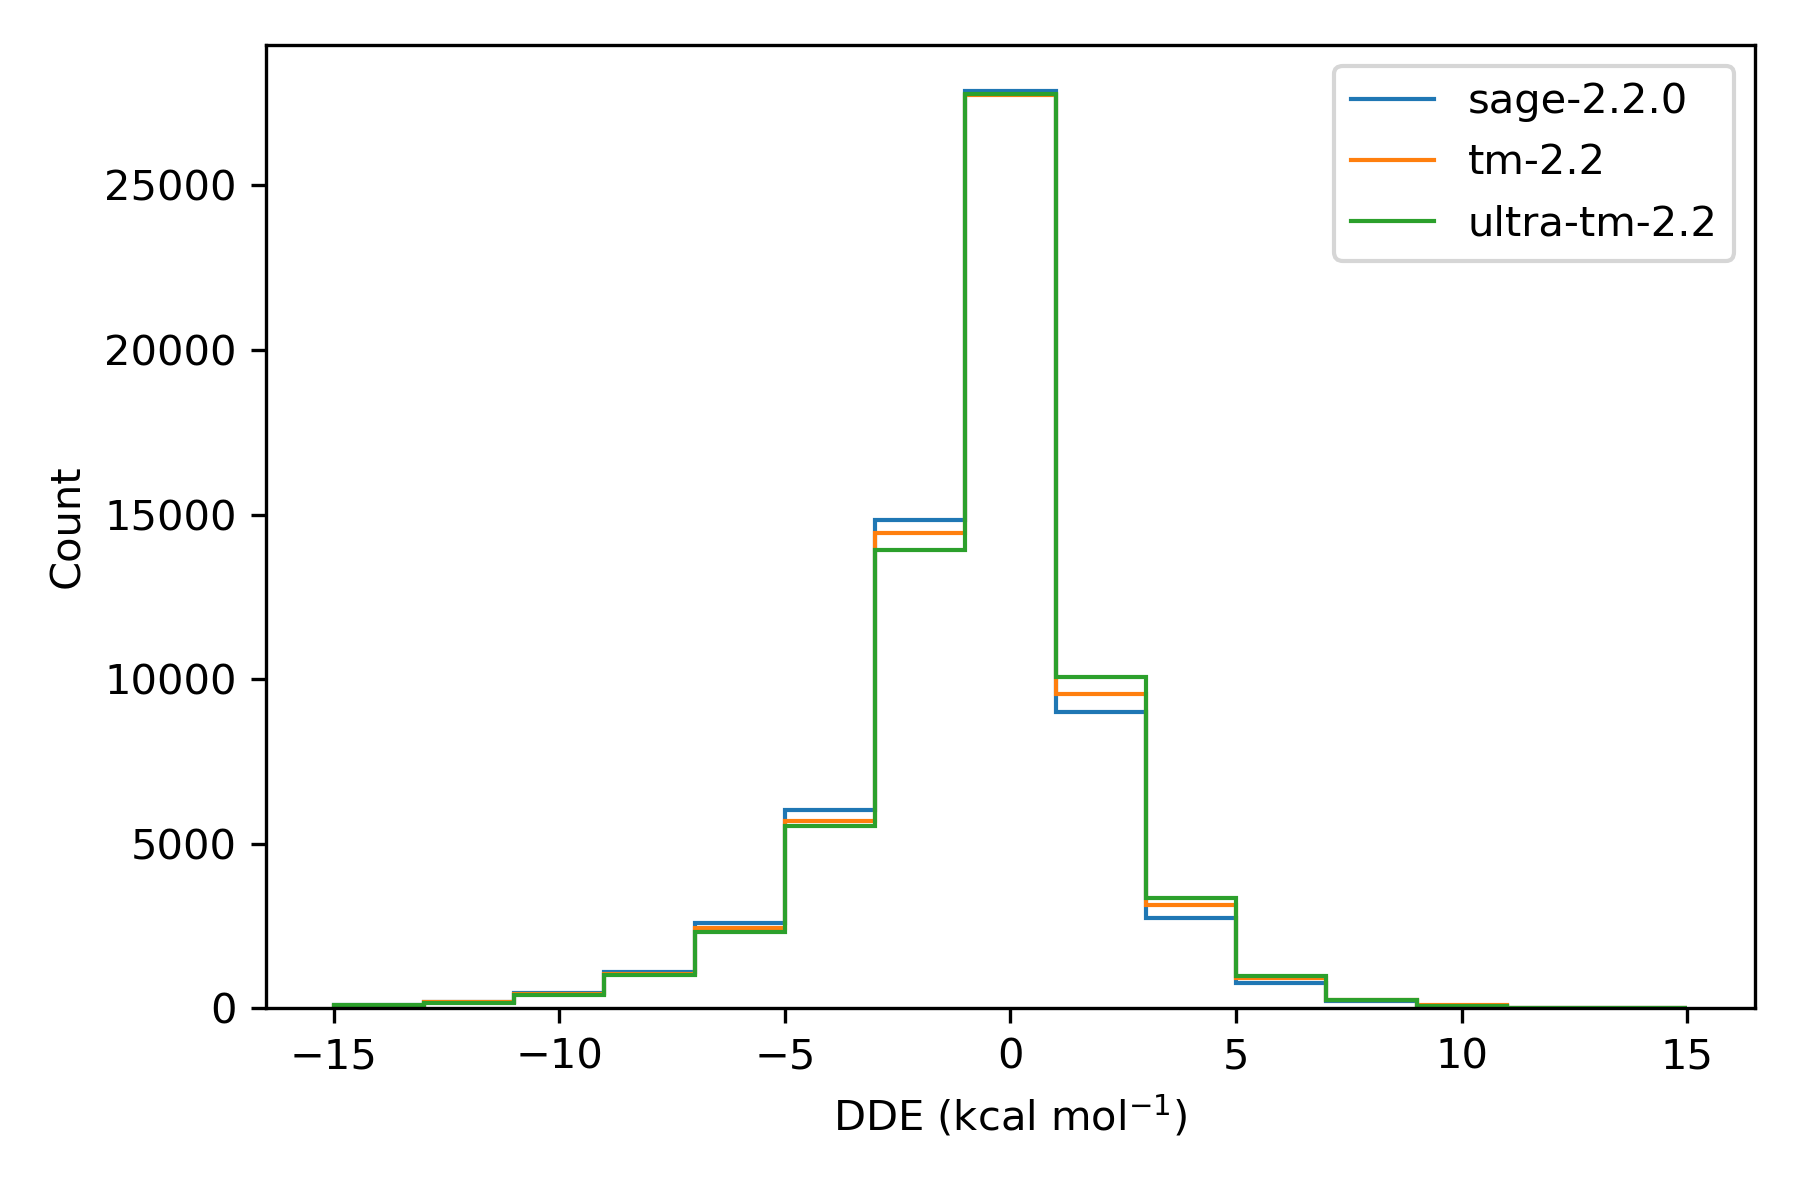
\includegraphics[width=0.49\textwidth]{figs/dde.png}
  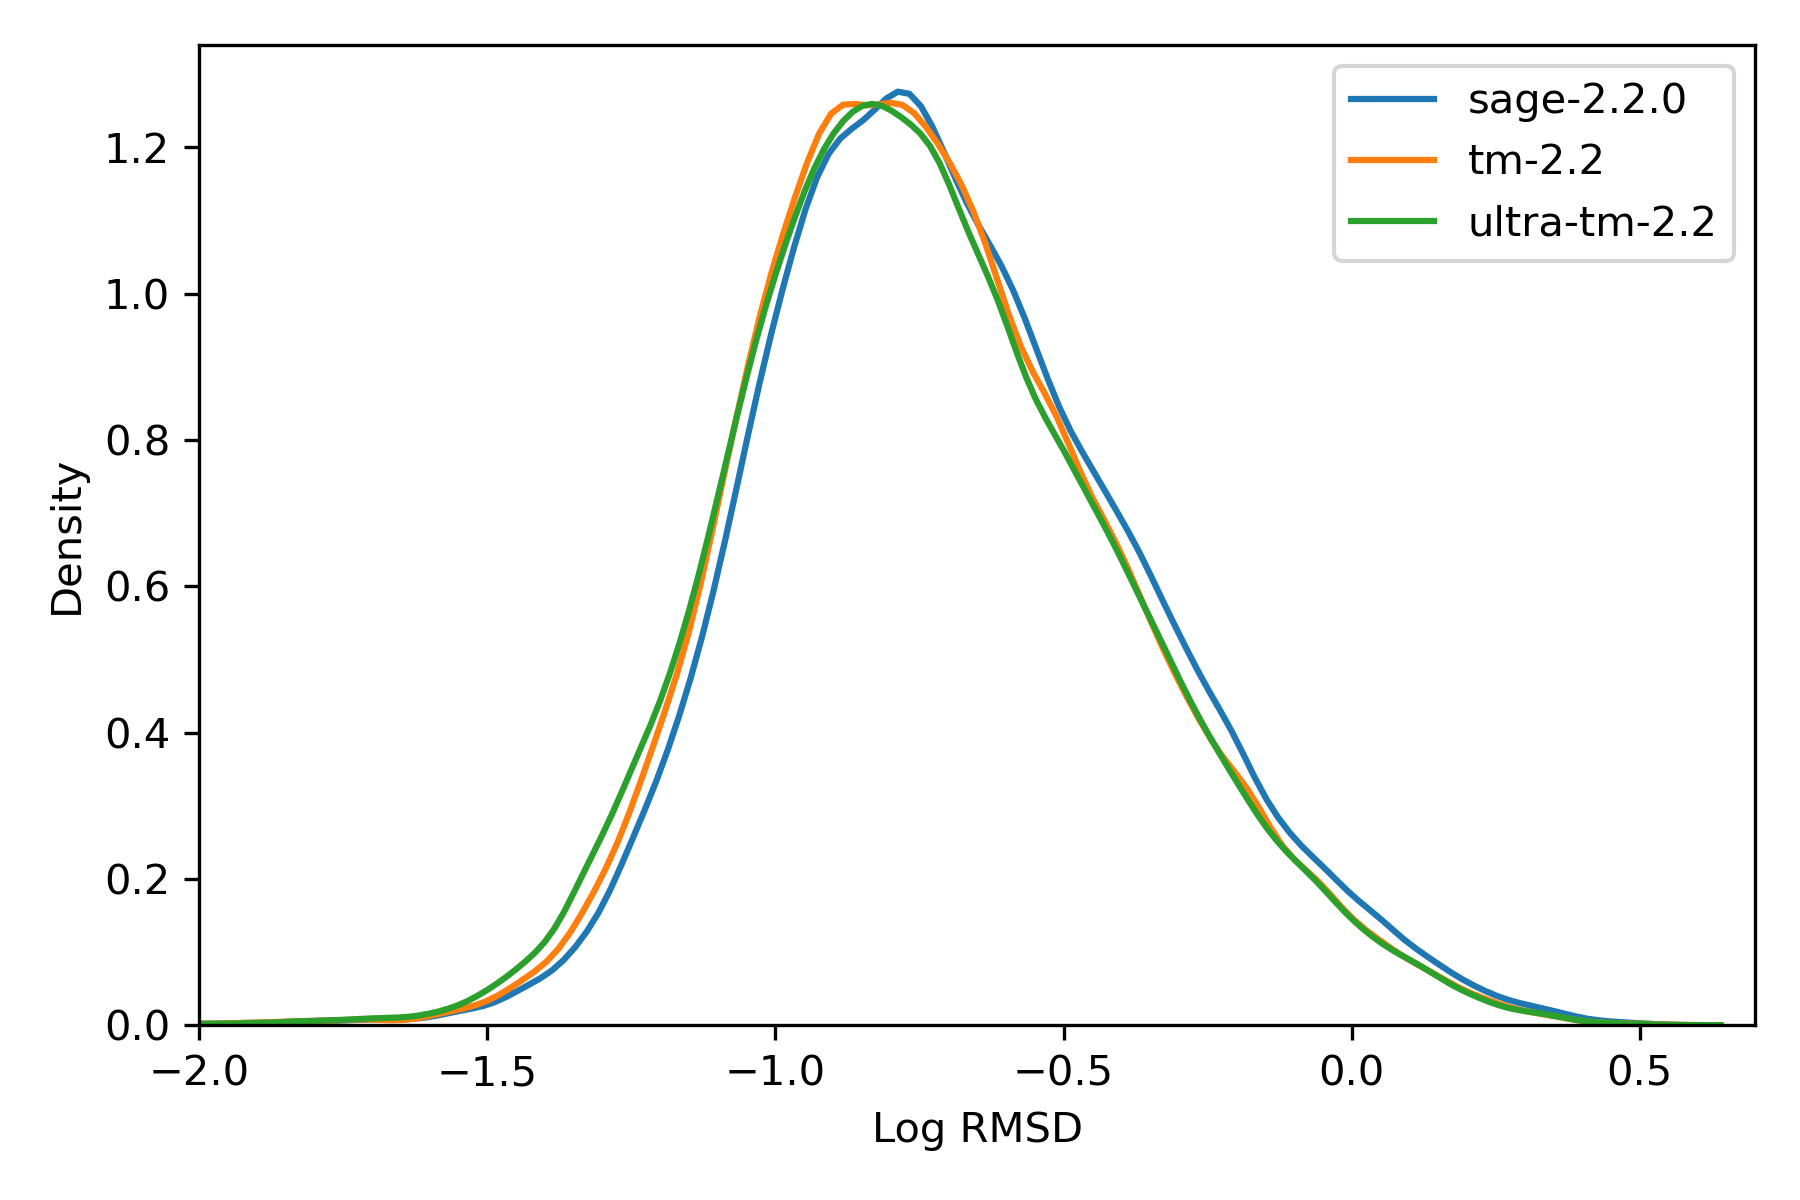
\includegraphics[width=0.49\textwidth]{figs/rmsd.png}
  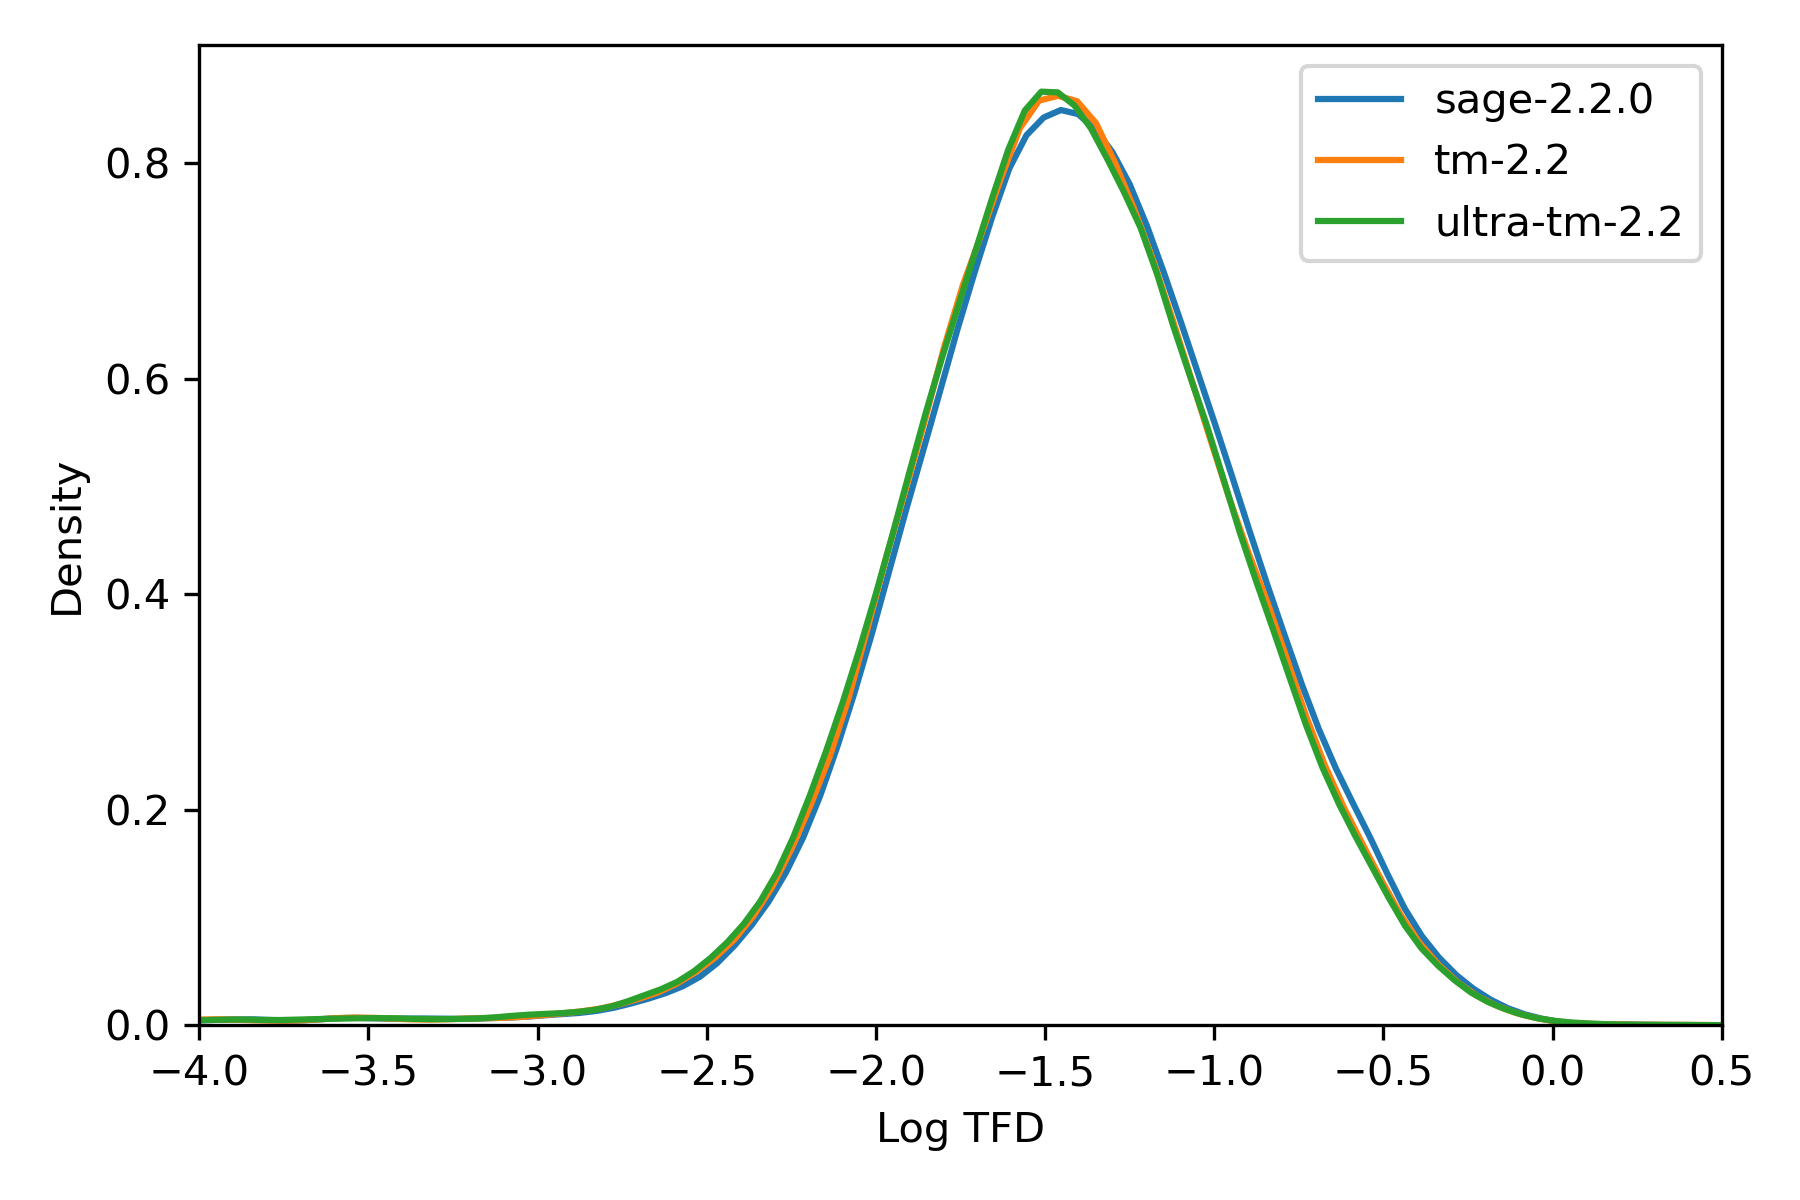
\includegraphics[width=0.49\textwidth]{figs/tfd.png}
\end{frame}

\begin{frame}
  \frametitle{DDE}
  \begin{center}
    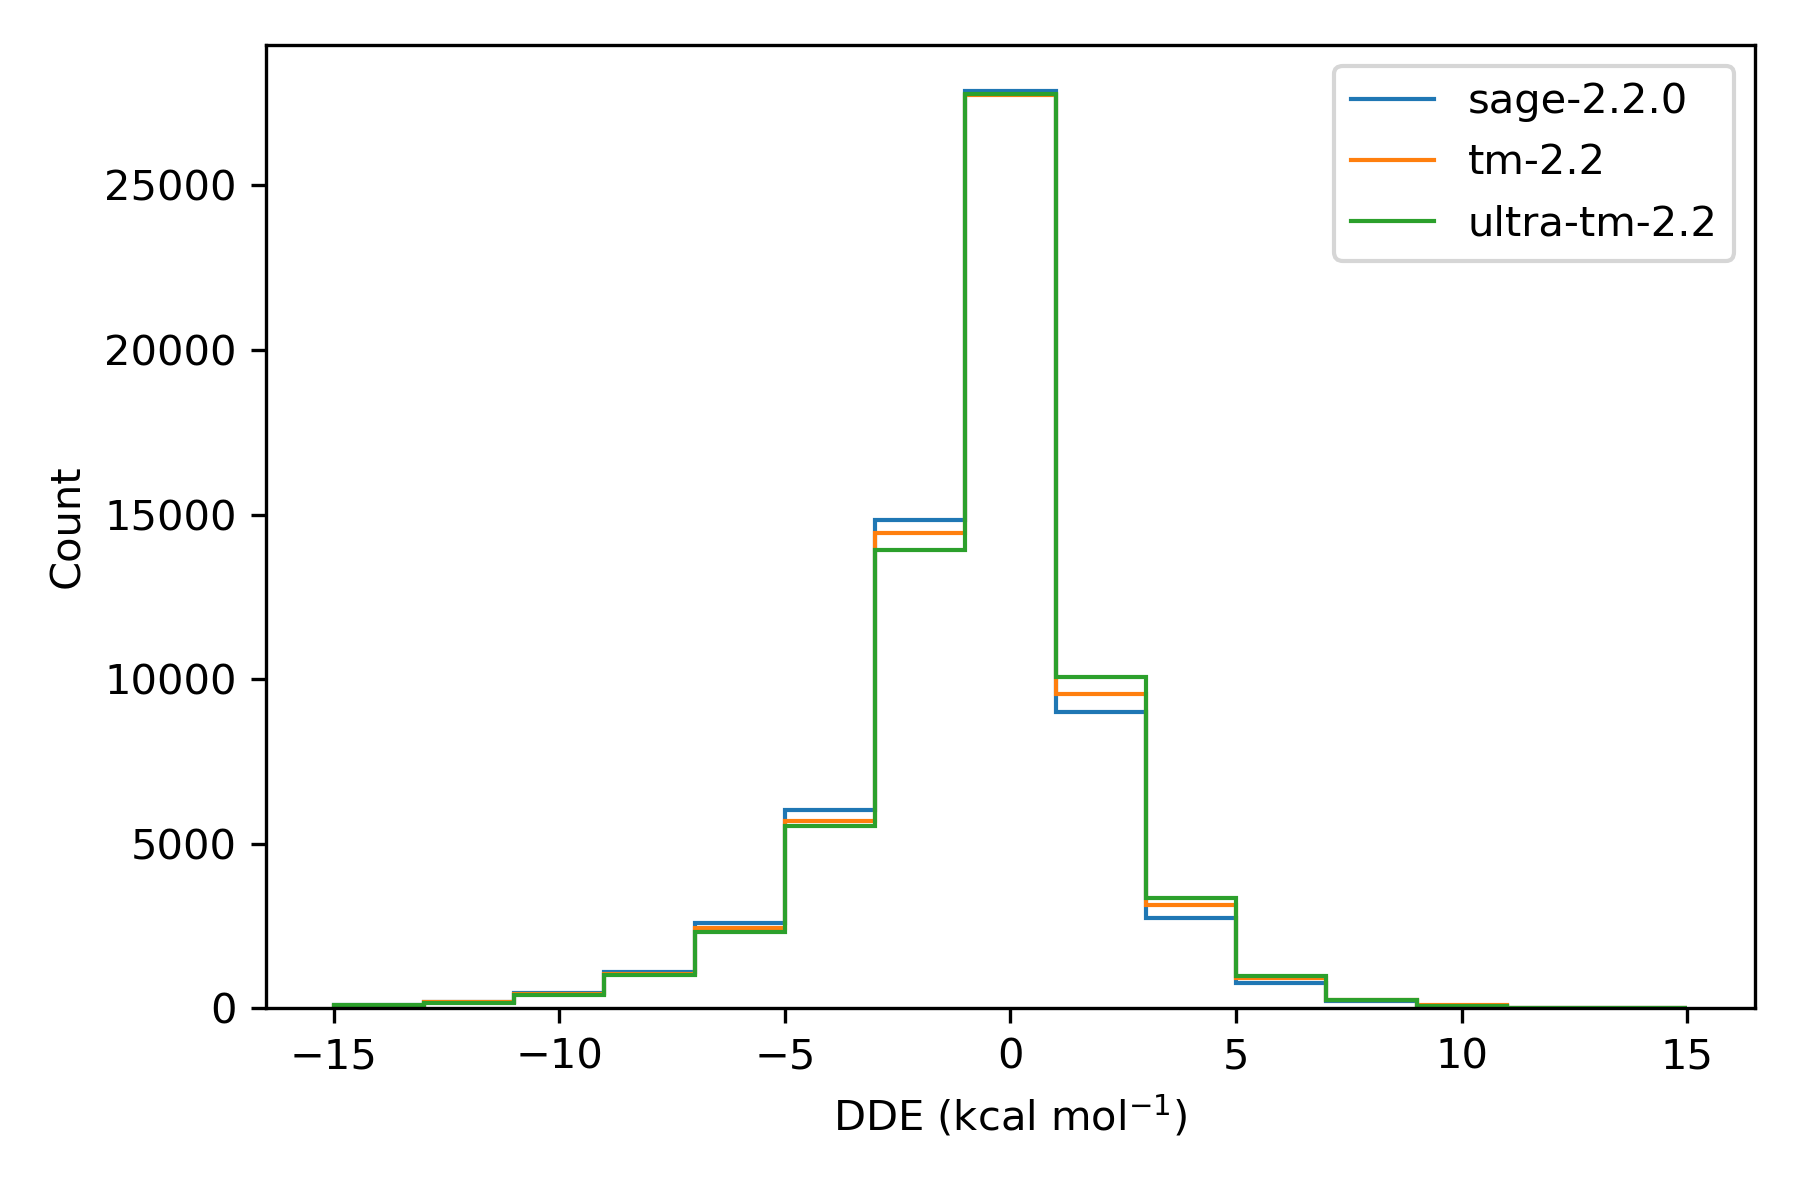
\includegraphics[height=0.8\textheight]{figs/dde}
  \end{center}
\end{frame}

\begin{frame}
  \frametitle{RMSD}
  \begin{center}
    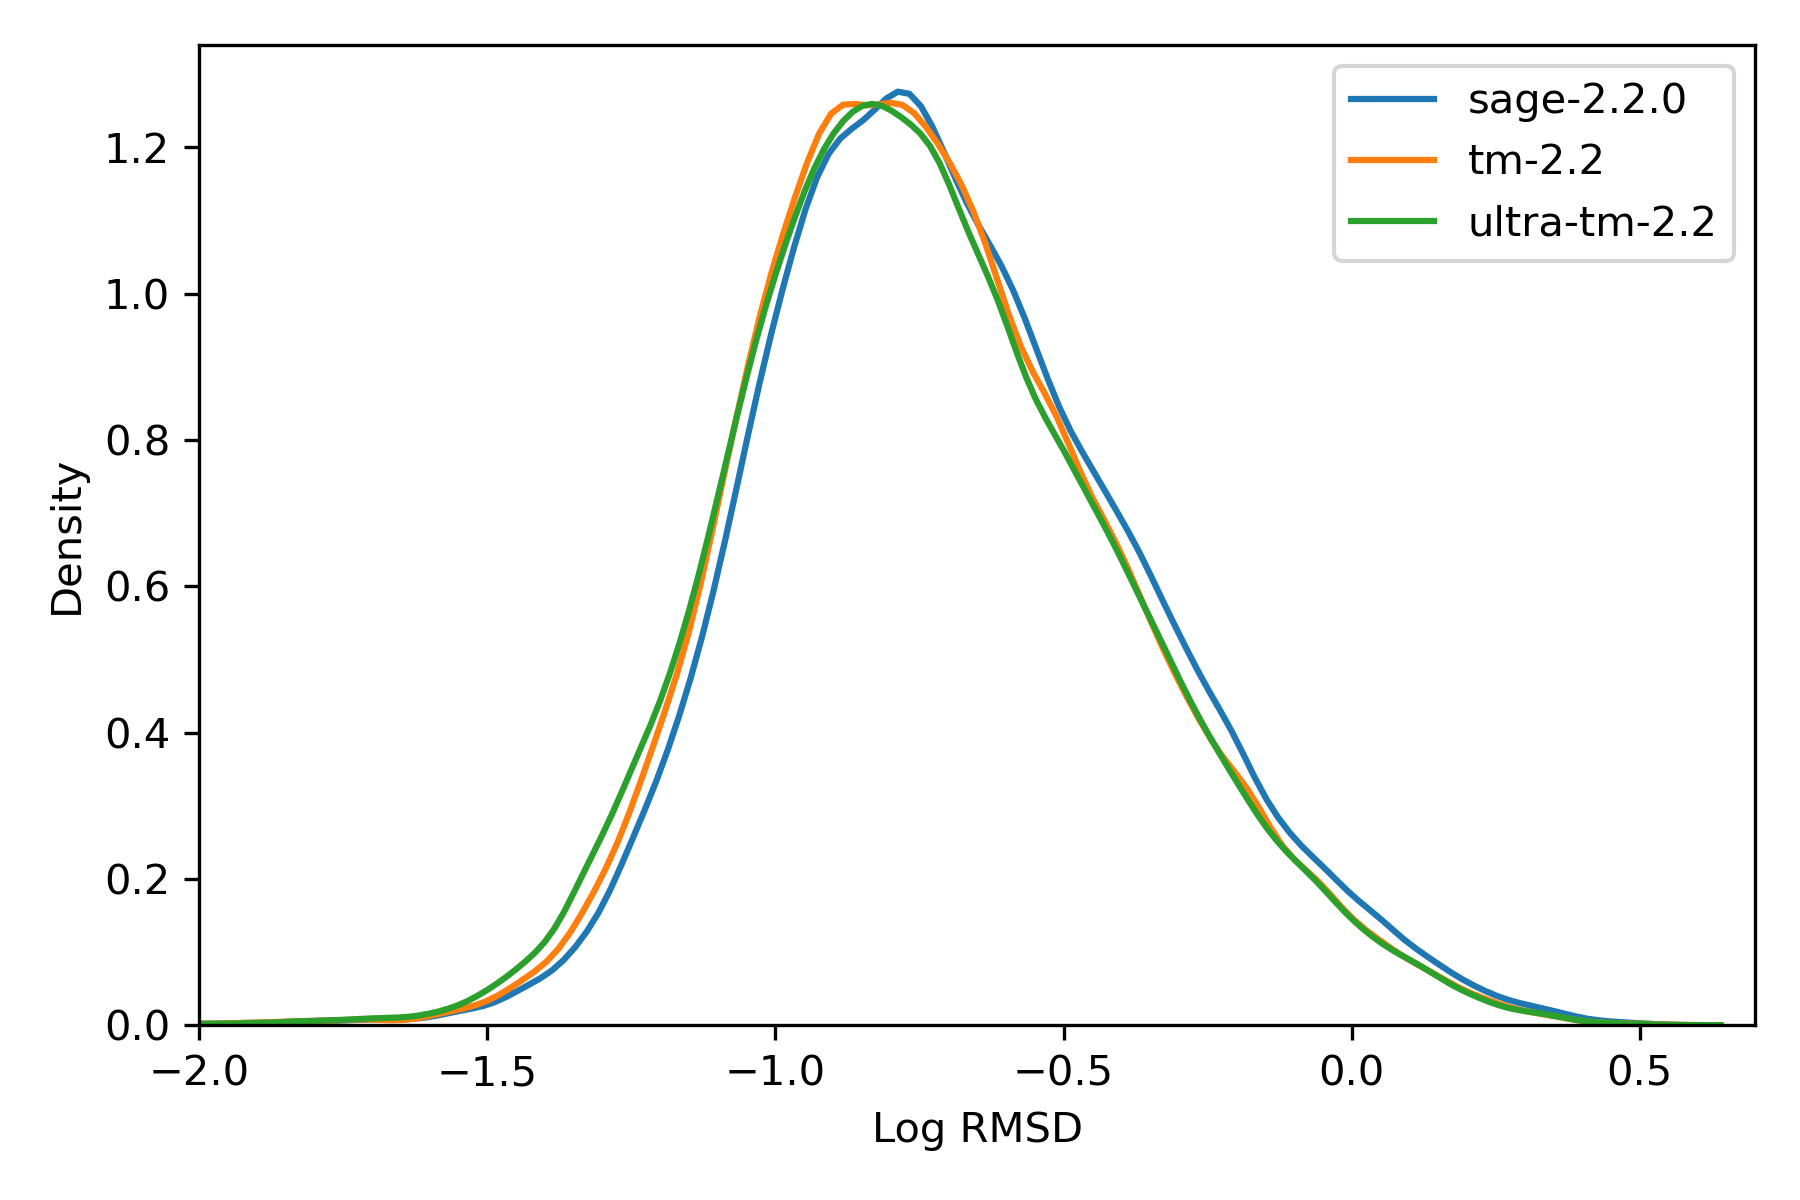
\includegraphics[height=0.8\textheight]{figs/rmsd}
  \end{center}
\end{frame}

\begin{frame}
  \frametitle{TFD}
  \begin{center}
    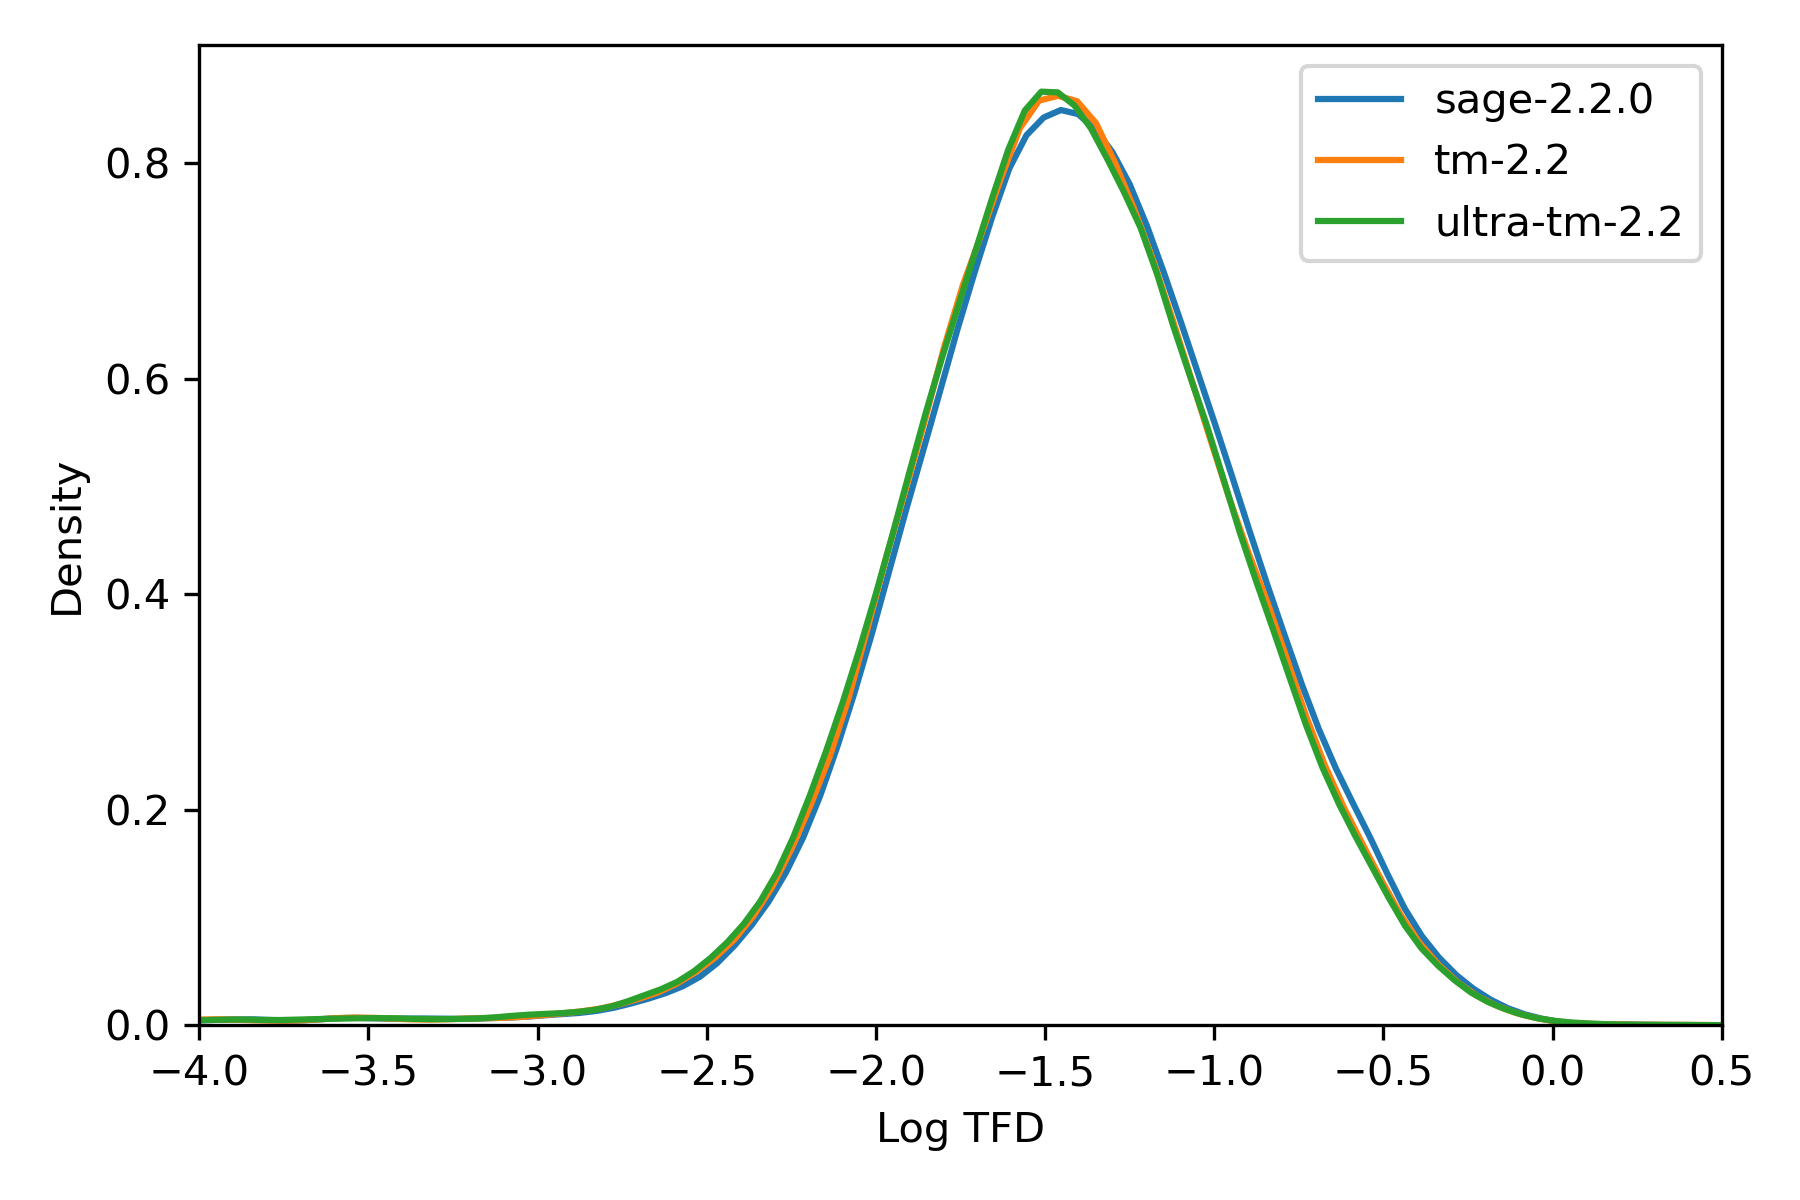
\includegraphics[height=0.8\textheight]{figs/tfd}
  \end{center}
\end{frame}

\begin{frame}
  \frametitle{Summary}
  \begin{table}
    \centering
    \begin{tabular}{llrrrr}
      Force Field & Metric & Avg & MAE & Mdn & SD \\
      \hline
      sage-2.1.0&DDE& -0.66 & 1.93 & -0.26 & 3.20 \\
smee-sage-2.1.0-opt&DDE& -3.50 & 12.37 & -2.24 & 25.54 \\
smee-sage-2.1.0-opt-td&DDE& -2.45 & 5.18 & -1.60 & 12.10 \\
\hline
sage-2.1.0&RMSD& 0.27 & 0.27 & 0.19 & 0.27 \\
smee-sage-2.1.0-opt&RMSD& 1.15 & 1.15 & 1.09 & 0.55 \\
smee-sage-2.1.0-opt-td&RMSD& 0.74 & 0.74 & 0.66 & 0.45 \\
\hline
sage-2.1.0&TFD& 0.07 & 0.07 & 0.04 & 0.09 \\
smee-sage-2.1.0-opt&TFD& 0.31 & 0.31 & 0.25 & 0.25 \\
smee-sage-2.1.0-opt-td&TFD& 0.17 & 0.17 & 0.12 & 0.16 \\
\hline

    \end{tabular}
  \end{table}
\end{frame}

\end{document}
